\chapter{Dask: a case of study for HPC in the cloud}\label{chpt:dask}

\section{What is Dask?}\label{sec:daskintro}

In the last two decades, the Python programming language has gained increasingly
more traction among the scientific community, becoming the de-facto standard in
many academic applications and research.
Consequently, many dedicated libraries have been developed to support the
researcher in their daily work.
Python is a very high-level language that is not designed with performances in
mind, and natively, it has minimal support to exploit the full potential of
multi-core CPUs or distributed systems.
This lack of native support is why all the libraries for scientific computing
are so important: implementing computationally demanding calls in more low-level
languages to achieve the best performance, these libraries provide the user with
a high-level interface to leverage the hardware's full potential, speeding up
computation.
Dask \cite{dask2015} is one of these libraries, first presented by Matthew
Rockling in 2015.

Dask is a flexible library designed to handle a wide range of applications, from
simple data manipulation to complex machine learning pipelines, in a parallel
fashion.
What makes Dask unique is that while most other scientific libraries aim to
exploit the full potential of a single machine by relying on a multi-core
architecture, Dask adds the ability to scale on multiple nodes, keeping all the
capabilities of efficiently using multi-threaded parallelism.
In a broader context, Dask is not the only library that provides distributed
computation; one notable example is \texttt{mpi4py} \cite{Dalcin2021}, a Python
wrapper for the MPI.
However, Dask meets the needs of the scientific community, as it provides a more
high-level interface without the need to deal with the complexity of the
communication aspect, which the library handles by itself at the possible cost
of a performance drop.
Dask is also greatly appreciated by the community, as it is actively developed,
maintained, and well-documented.
Another reason for the popularity of Dask is the low entry barrier, which makes
the library usable by even the less expert Python programmers.
There is no need to use things like classes and objects and adopt an
object-oriented programming style, as the library is designed to be used in a
functional programming style, using structures more similar to tuples, lists,
and dictionaries  \cite{dask2015}, making it a more attractive choice for the
adoption in a scientific project.

The idea behind Dask is to encode the program's code into a directed acyclic
graph (DAG), built as a dictionary by the library itself, where each entry is a
task to be executed.
This object is then passed to the \textit{``scheduler''}, the component
responsible for managing the computation graphs, and the \textit{``workers''}:
the components that perform the computation.
The scheduler is a crucial library component and represents one of the most
impactful choices in terms of total overhead introduced.
By default, the scheduler adopt a ``last in, first out'' (LIFO) strategy,
meaning that the next task to be executed is the one whose dependencies were the
most recently resolved.
The idea behind this choice is to keep the scheduler as simple as possible,
avoiding spending too much time computing complex metrics to decide the next
task to schedule and keeping the overhead as low as possible.
Several scheduler implementations are available depending on the use case, like
a single-threaded, multi-threaded, or multi-process mode.
Since the impact on the final performance of the scheduler is significant, many
efforts have been made to find a more efficient implementation\cite{bohm2020}.
In any case, the scheduler is a replaceable component, and the user can
implement its scheduler tuned for its specific use case.

The scheduler submits the tasks to the workers responsible for the computation,
who then report the results to the scheduler.
Workers need to access the shared filesystem or a shared data source, but they
are agnostic about the physical location where they are running.
This means that the workers can run on the same machine where the scheduler is
running or on different machines in a distributed environment, making the
parallelism of the execution implicit and transparent to the user.
Furthermore, this distributed nature allows for high fault tolerance, as the
number of workers can change dynamically.
If some cannot reach a certain point, they will not receive any task to perform.

\section{Dask in practice}\label{sec:daskcloud}

To enable efficient computation in different situations, Dask introduces several
abstractions to simplify parallel computing tasks.
At its core, the library offers three primary collections: Dask-Arrays,
Dask-DataFrames, and Dask-Bags.
Those collections mime perfectly the interface of some of the most popular and
widely used libraries in the scientific community, like NumPy and Pandas, making
the transition to Dask very smooth for the user.

\begin{itemize}
  \itemsep0em
  \item \texttt{dask.array}: provides a subset of the trendy NumPy library,
    keeping the same interface.
    It is designed to operate with multi-dimensional arrays of numerical data
    that can be partitioned across multiple nodes in the cluster.
    Each partition is called a \texttt{chunk} or \texttt{block} of data, which
    Dask can process in parallel.
    This allows users to work with data that does not necessarily fit in the memory
    of a single machine\cite{daskdoc-array}.

    This object is the less structured collection, which is meant for numerical data.
    For this reason, it is also the most efficient one and comes with many
    functions to manipulate the already implemented and optimized data.
  \item \texttt{dask.bag}: is an unordered collections which allows repetitions.
    It is meant to be used with unstructured or semi-structured data.
    They are suitable, for example, for large-scale data processing tasks such
    as natural language processing.
  \item \texttt{dask.dataframe}: provides the same interface as the popular
    Pandas library, which is widely used for data manipulation.
    It is meant to be used with structured data, in detail, with tabular
    data\cite{daskdoc-dataframe}.

    However, since the data are more structured and can be more heterogeneous,
    for instance, numerical and strings data in various columns far from the one of
    the Dask-Array\cite{dask2015}.
\end{itemize}

Since its first release, the interest in the project has grown, and the
community has developed several extensions to the library for specific
applications or environments, like Dask-ML or Dask-CUDA for ML applications or
the \texttt{dask\_jobqueue} and \texttt{dask-kubernetes} to interface with
existing resource manager systems.

The first one, \texttt{dask\_jobqueue}, is designed to facilitate using Dask in
traditional HPC clusters.
This package simplifies the creation and management of Dask clusters (set of
scheduler and its workers) on these systems by providing an interface that
abstracts much of the complexity of configuring and launching jobs across
multiple nodes.
It provides an interface to uniformly allocate the resources on the cluster,
such as setting parameters like the number of workers and the assigned resources
(CPUs and memory); this library autonomously submits the job to the cluster's
job scheduler.
This way, the user can focus on the computation without worrying about resource
allocation, which may vary depending on the adopted scheduler (SLURM, PBS, LSF,
and many others are supported).
In this way, multiple jobs will be autonomously spawned, each executing the
\texttt{dask-worker} command, which will connect to the scheduler and start to
execute the tasks.
The worker will be automatically terminated when the computation finishes and
the resources are released.

The latter one, \texttt{dask-kubernetes}, is tailored for modern cloud-native
environments where applications are containerized and orchestrated by
Kubernetes.
This package interacts with a dedicated \texttt{dask-operator}, which must be
installed on the cluster.
It creates the appropriate manifest containing a DaskCluster resource on the fly
to apply to the Kubernetes cluster.
The user can specify the number of workers and the resources to allocate, and
the operator will create the pods and the services needed to execute the
computation.
It is also possible to specify the image for schedulers and workers if the user
wants to use a custom image with some specific libraries installed.

Overall, Dask's design and supporting ecosystem provide a versatile and scalable
platform for parallel computing, whether on a single machine, a traditional HPC
cluster, or a modern cloud infrastructure.
This flexibility and its compatibility with familiar Python tools make Dask an
appealing choice for data scientists, researchers, and engineers looking to
handle large-scale data processing and computation efficiently.

\section{Benchmarking Dask}\label{sec:daskbenchmark}

Being versatile and flexible, we believe Dask is the perfect tool for assessing
how a given infrastructure performs under various workloads.
This section will present a benchmark developed with Dask that aims to simulate
some operations commonly executed in a scientific context.
Similarly to the previous chapter, the idea is to execute the same code on the
two nodes of the THIN partition of ORFEO cluster\ref{sec:measurements}
provisioned with the SLURM job scheduler.
Then, the same code will be executed on the same hardware, but the Kubernetes
orchestrator will be used to manage the resources in this second iteration.
Since the code is the same, the only difference between the two executions is
how the resources are allocated and managed, which will allow us to
quantitatively determine the performance gap between the two different cluster
management paradigms.

Since we could not find an exhaustive and recognized benchmark to measure Dask's
performance and wanted to control the code and the operations executed, we
developed a code specifically for this purpose.
The proposed benchmark is a collection of operations commonly executed in
scientific contexts and designed to be executed on arrays and data frames.
The code base is heavily inspired by a blog post by Matthew Rocklin, where he
presents a similar benchmark to show Dask's scalability performance and
limits\cite{Rocklinblog}\footnote{
  Our benchmark source code is available in this git repository
  \url{https://github.com/IsacPasianotto/dask-bench}
}.

\subsection{Tasks description}\label{subsec:benchmarktasks}

The code is designed to evaluate the so-called ``weak scalability'', which means
that the data size is scaled according to the number of computational resources
used, keeping the amount of data per worker constant.
The ideal case for weak scalability is when the execution time remains constant,
regardless of the number of workers used, or equivalently, the rate of data
processable per unit of time is a linear function of the number of workers.
For what concerns the operations executed on the arrays, the benchmark is
composed of the following tasks:

\begin{itemize}
  \itemsep0em
  \item \textit{Randomly initialization of a 2-D array}: It measure the time
    needed to randomly initialize a 2-D array of integers representing a
    $\psi\times\psi$ matrix and persist it in memory.

    The size $\psi$ of the array is scaled accordingly to the number of cores
    used, with the following formula: $\psi = k \cdot \sqrt{n}$ where $k$ is a
    constant term fixed to 5000 and $n$ is the number of cores used.
  \item \textit{``blockwise'' operation}: To efficiently store and manipulate
    the arrays, Daks split the data into blocks, the smallest data unit that
    can be processed in parallel.
    The library provides a function \texttt{map\_blocks()} that applies a
    function to each block of the array.

    The elementary function \texttt{x += 1} is used in this case.
    This is an embarrassingly parallel operation since no communication is
    needed, making it a perfect candidate to see the impact of the overhead
    given by the scheduler-worker communication.
  \item \textit{``elementwise'' operation}: Similar to the previous case, but in
    this case, instead of relying on the block structure of the array, a new
    array is created, and its elements are computed sequentially one by one:
    \texttt{y = sin(x)**2 + cos(x)**2}.
  \item \textit{reduction operation}: The variance of all the array elements is
    computed.
    This is a reduction operation, meaning the result is a scalar value computed
    from the whole array.

    Unlike the previous case, this operation requires a little communication
    since the workers must communicate with each other (passing through the
    scheduler) the partial results to compute the final one.
 \item \textit{``row-wise'' reduction operation}: Similar to the previous case,
   but in this case, the variance is computed for each row of the array.
    This operation is more complex than the previous one since it requires more
    communication, and the final result is a 1-D array of the same length as the
    original array's number of rows.

    Note that since the array is stored partitioned by blocks, which can be
    visualized as sub-matrices, elements of the same row reside in different
    blocks, which can be assigned by the scheduler to different workers, making
    the communication more relevant.
  \item \textit{Random access}: It measures the time needed to retrieve a single
    element at an arbitrary position of the array.
    This operation is not parallelized, and the expectation is that the time
    needed to retrieve an item should remain constant regardless of the number
    of workers used.
  \item \textit{Sum of the transposed matrix}: Compute the sum of the original
    matrix with its transpose $B = A+A^T$.

    This task is more complex and is meant to be an example of a more
    sophisticated computation that requires more communication since the
    corresponding symmetric entries must be retrieved for each element of the
    matrix.
\end{itemize}

Instead, for the data frame, the operations are:

\begin{itemize}
  \itemsep0em
  \item \textit{Randomly initialization of a dataframe}: Time needed to
    initialize a  \texttt{dask.DataFrame} with $6$ columns and $\varphi$ rows.
    In this case, since the number of columns is fixed, to keep the ratio of the
    problem size and the number of workers constant, the number of rows is
    scaled linearly with the number of workers: $\varphi = k \cdot n$ where $k$
    is a constant term fixed to $3000$ and $n$ is the number of cores used.
    Although the DataFrame is a more structured object that allows storing
    different types of data, all columns are filled with random integer numbers.
    The reason is to keep the benchmark as simple as possible and to maximize
    the number of operations done in the following steps (since some of those
    can only be performed for numerical data).
  \item \textit{``blockwise'' operation}: similarly to the array case, the
    \texttt{map\_partition()} function provided by the Dask library is used to
    compute a new DataFrame where each element is incremented by one.
  \item \textit{Random access}: A fixed dataframe row is retrieved.
    Like in the analog array case, the expectation is that the time needed to
    retrieve a row should remain constant regardless of the number of workers.
  \item \textit{Reduction operation}: Measure the time needed to compute a
    reduction operation (standard deviation) over all the numeric columns of the
    data frame.
  \item \textit{``group-by'' with reduction, 1 column}: The group-by operation
    is a typical operation in data manipulation and processing. Given a data
    frame, it will return a new data frame where all the rows with the same
    value over a specific column are grouped together.
    The result is a new row with the share value in the column taken as
    reference and the result of a reduction operation (in this case, the
    standard deviation) over all the other columns.
  \item \textit{``group-by'' with reduction, 2 columns}: Analogue to the
    previous case, but in this case, the rows will be grouped by the values of a
    pair of columns.
  \item \textit{Sort the data}: Time needed to re-arrange all the data frame
    rows such that the values of a given column are sorted.

    This scenario is expected to be the one that involves the most communication
    among the workers since the rows must be re-arranged in a specific order.
\end{itemize}

\section{Results and analysis}\label{sec:daskresults}
\subsection{Data collection}\label{sec:daskresults}

The code was executed on two nodes of the THIN partition using the
\texttt{dask\_jobqueue} and \texttt{dask-kubernetes} packages previously
mentioned. The baseline for the serial execution was collected with 1 core.
Then, data points were collected by increasing the number of cores from 2 to 48
with a step of 2; being 48 the number of cores of the combined two nodes.
These operations were performed in both cases, bare metal and Kubernetes with
Cilium CNI for pod communication.
Only the worker processes were executed in the two nodes dedicated to the
computation to retain all the resources in the computational nodes for the
actual benchmark.
The scheduler was executed on a different node equal to the previously mentioned
THIN nodes.
The benchmark was run thirty times for each configuration, and the average time
with the standard deviation was computed to have a more reliable estimation of
the performance of the infrastructure.
In all the cases, all the computational resources used were taken exclusively
for the measurements, ensuring that no other processes that could interfere were
running on the same nodes.

In the bare metal case, the SLURM job scheduler makes allocating the resources
straightforward since it allows for specifying the number of CPUs to book a job
and then spawn the processes in the allocated resources. It is sufficient to
submit multiple jobs with the same amount of CPUs and memory requested, one for
each worker used, to have the desired configuration.

In Kubernetes, this process is more complex.
One of an orchestrator's most important and characteristic features is the
ability to manage the resources dynamically.
This behavior, which usually is a great advantage, must be disabled in this
case; otherwise, as soon as the pod is created and the scheduler realizes that
it is saturating the initially assigned resources, it will try to allocate more,
resulting in the invalidation of the measurements since the final results will
not be comparable anymore.
However, the Kubernetes API offers a way to specify the resources that a pod can
use.
In particular, the \texttt{spec.container.resources.limits} and
\texttt{spec.container.resources.requests} fields serve this purpose
\cite{kdoc-resources}.
The \texttt{requests} field specifies the minimum amount of resources a pod
needs to find available in a node to be scheduled.
If not enough resources are available, the pod will remain in the pending state
until the resources are freed.
The \texttt{limits} field is used to specify the maximum amount of resources
that a pod can use in case of need.
This does not mean that the resources specified in this field are reserved for
the specific pod; in fact, it is possible to ``overbook'' the resources of a
node, for example, in the case of different workloads on different pods are
executed simultaneously but require more resource in a disjoint time intervals.

To obtain a fair comparison and mimic the behavior of the SLURM job scheduler
with kubernetes, it is sufficient to set the \texttt{requests} and
\texttt{limits} fields to the same values.
This way, the amount of resources needed by the pod will be reserved, and the
pod will not be able to use more.
Eventually, the \texttt{spec.replicas} field is used to specify the number of
replicas of the pod that must be created.

The criteria used to decide the amount of resources to allocate for each worker
remain to be specified.
There is no general rule to follow, and preliminary analysis showed that
different configurations can lead to better performance in some cases and worse
in others.
The adopted strategy was to set:

$$
\#_{\text{worker\_CPUs}} = \left\lfloor \frac{\#_{\text{CPUs}}}{\left( \left\lfloor
    \frac{\#_{\text{CPUs}} - 1}{\#_{\text{CPUs\_per\_node}}} \right\rfloor \right) + 1} \right\rfloor
$$

\noindent where $\#_{\text{worker\_CPUs}}$ is number of CPUs assigned to each
worker $\#_{\text{CPUs}}$ is the number of requested CPUs for the computation
and $\#_{\text{CPUs\_per\_node}}$ is the number of CPUs available on a node.
Through this strategy, first, a node will be filled up to the maximum available
CPUs (in the case of the used hardware: 24 cores), using a single worker.
Then, once the number of used cores is greater than the number in a node, a new
worker will be spawned, splitting the global amount of booked CPUs among the
workers in equal parts.
This choice aims to achieve the best performance by eliminating infra-node
communication and keeping only the unavoidable inter-node one.

An observation that must be made is the difference in how the SLURM scheduler
and Kubernetes orchestrator let the user allocate the requested resources.
The first considers 100\% of the hardware resources bookable for a job, while
the latter has a minimum amount of resources that must be reserved for itself.
Clearly, the Kubernetes approach is the correct one, as SLURM itself is not
exempt from having system processes (like the daemon itself) running on the same
nodes and inevitably consuming some resources.
This could seem a small detail, but it has the consequence that the total amount
of bookable resources in Kubernetes results to be less than 100\% of the
hardware resources.
As a consequence, during the execution of the described benchmark, when the
cores assigned to the pod worker are close or equal to the total available on
the node, Kubernetes will start to throttle the pod since the pod will be
considered un-schedulable.
For this reason, results presented in the following sections obtained with
Kubernetes will have fewer points.

Similar to the previous chapter, due to the large amount of data generated by
the experiments, only a subset of these will be presented in this thesis.
The complete set of results can be found in a supplementary report \footnote {
  The supplementary material can be obtained at the following link
  \url{https://github.com/IsacPasianotto/master-thesis/blob/main/appendixC-dask_results/report.pdf}.}.
Also, as in the previous chapter, the following pages will present the results
of the benchmark graphically to make them more readable and more accessible to
be interpreted\footnote{Detailed numerical results will be reported in appendix
\ref{appendix:dask}}.


\subsection{Arrays}

The obtained results confirm the expectations that the array is the most
performant collection of Dask: the scaling is quite satisfactory, and the time
to execute the operation, even if it increases, does not explode like in the
data frame case.

The findings corroborate the hypothesis that the performance of a container
orchestrated by Kubernetes is absolutely comparable to that of a job executed in
bare metal with traditional HPC tools.
The performance gap is negligible, and the results are almost identical. This
should instill confidence in the comparison we've made.

Also, in where a modest amount of communication is needed, like the case of
row-wise reduction computation reported in figure
\ref{fig:array-reduction-std-along-axis}\footnote{
  Data are available in tables \ref{tab:baremetal-reduction-(std)-along-axis}
  and\ref{tab:kube-reduction-(std)-along-axis} in appendix \ref{appendix:dask}.
}, the performance are absolutely comparable and the overhead introduced by the
Kubernetes orchestrator is negligible. The difference in the plotted points is
more likely due to the intrinsic variability of the execution time of the tasks
rather than to the different infrastructures used under the hood.

The story changes when the workers' communication is more relevant, becoming the
dominant aspect of the performed operation.
We can see in the figure \ref{fig:array-sum-transposed-matrix}\footnote{
  Data are available in tables \ref{tab:baremetal-sum-the-transpose} and
  \ref{tab:kube-sum-the-transpose} in appendix \ref{appendix:dask}.
} how in the case of the sum of the transposed matrix, in the Kubernetes case,
the rate of data processable per second drops immediately when the number of
cores exceeds 24, forcing the scheduler to allocate the workers on different
nodes and to exchange data among both of them continuously.
In this specific case, the whole infrastructure of Kubernetes, in particular for
the connectivity aspect handled by the Cilium CNI, is not able to keep pace with
the bare metal case, where communication is more efficient and faster.
In this case, the difference is absolutely not negligible.

\begin{figure}
  \centering
  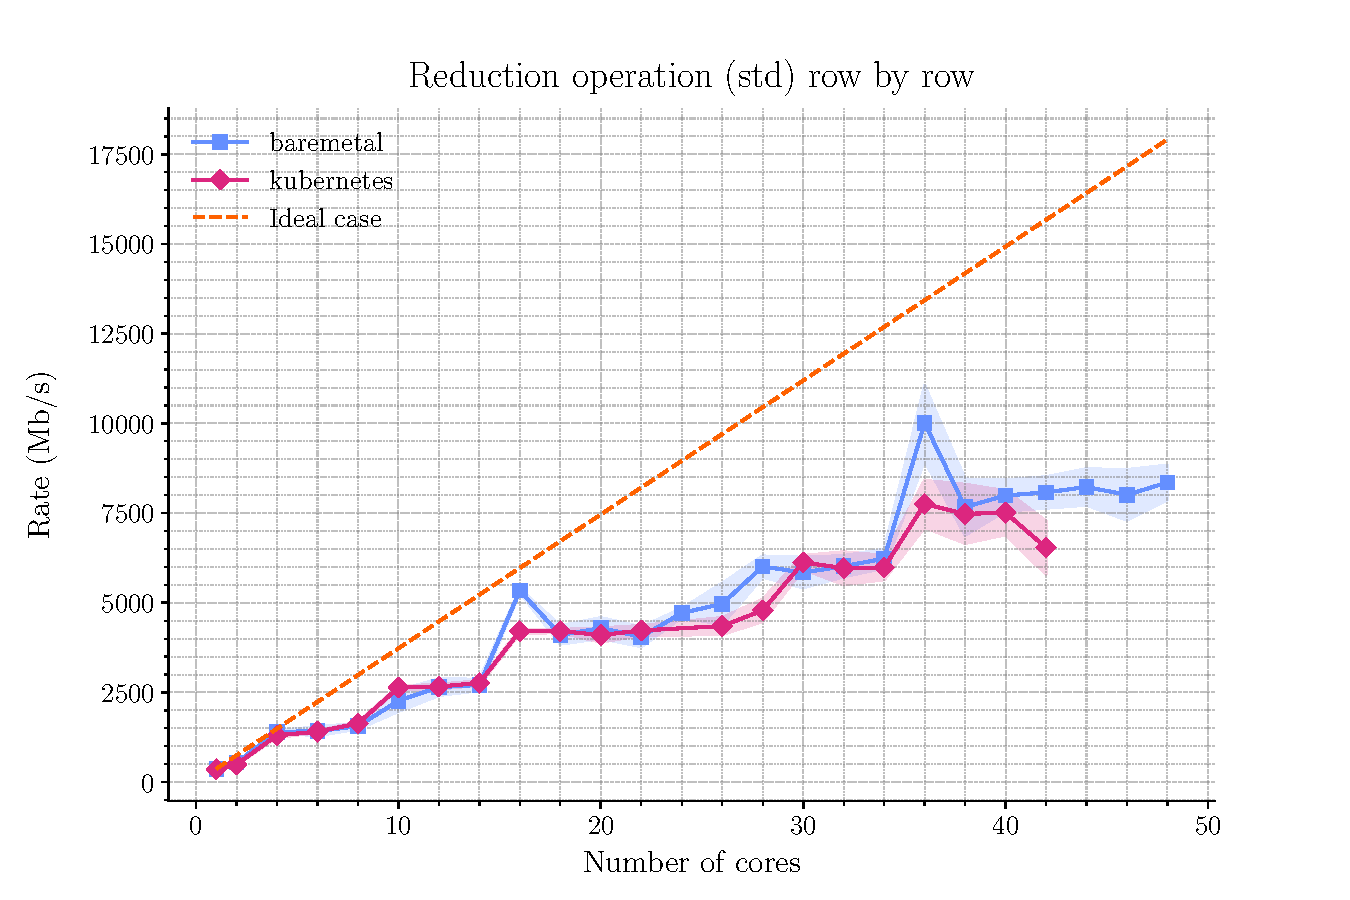
\includegraphics[width=0.9\textwidth]{img/chpt4/array-reduction-std-along-axis}
  \caption{Disparity in performance between the bare-metal setup and the
    Kubernetes cluster on equivalent hardware while carrying out a row-wise
    reduction operation on a 2-D array.}
  \label{fig:array-reduction-std-along-axis}
\end{figure}

\begin{figure}
  \centering
  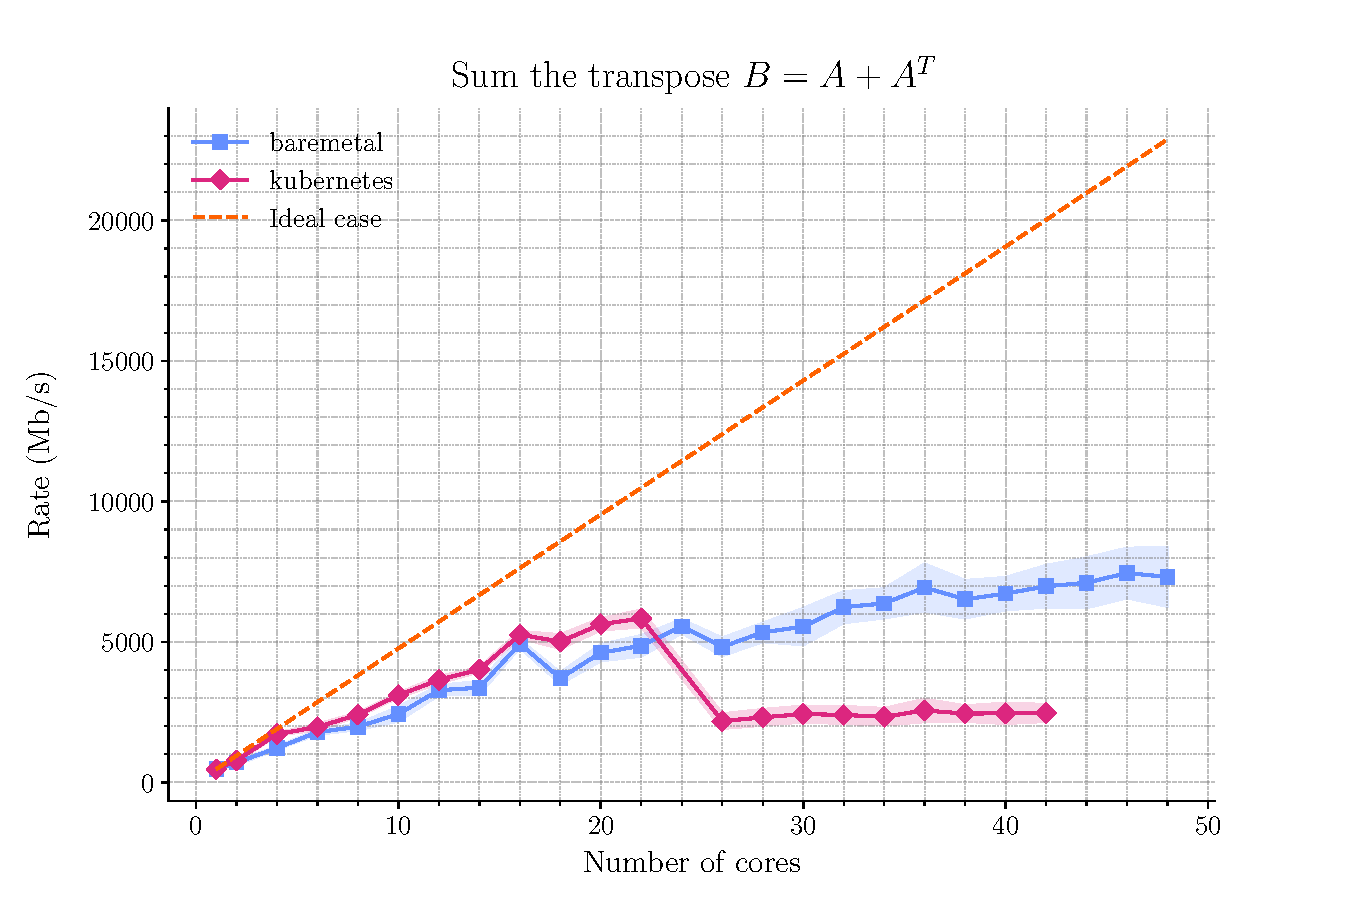
\includegraphics[width=0.9\textwidth]{img/chpt4/array-sum-the-transpose}
  \caption{Difference in performance between the bare metal case and the
    Kubernetes cluster on the same hardware in performing the sum of a matrix
    with its transpose $B=A+A^T$.}
  \label{fig:array-sum-transposed-matrix}
\end{figure}

The measurements taken on the time needed by retrieving an element from a random
position in the array, represented in figure{fig:array-random-access}\footnote{
  Data are available in tables \ref{tab:baremetal-random-access} and
  \ref{tab:kube-random-access} in appendix \ref{appendix:dask}.
}, are fascinating.
In the ideal case, the time is supposed to be constant, and the faster or slower
communication between the workers and the scheduler causes any difference
between the results of the two infrastructures. As was predictable, the
Kubernetes case is slightly slower than the bare metal one.
The difference is not too impactful, with just one node involved. At the same
time, the gap becomes wider after the 24 cores, when the workers are allocated
to different nodes, and the communication becomes more relevant.

An interesting behavior not spotted in other cases is the significant the
difference in variability the two infrastructures have: the Kubernetes case is
way more variable than the bare metal one, meaning that even if, on average, the
performance is lower than the bare metal case, in some cases the Kubernetes may
be faster than the bare metal unlucky case.

\begin{figure}
  \centering
  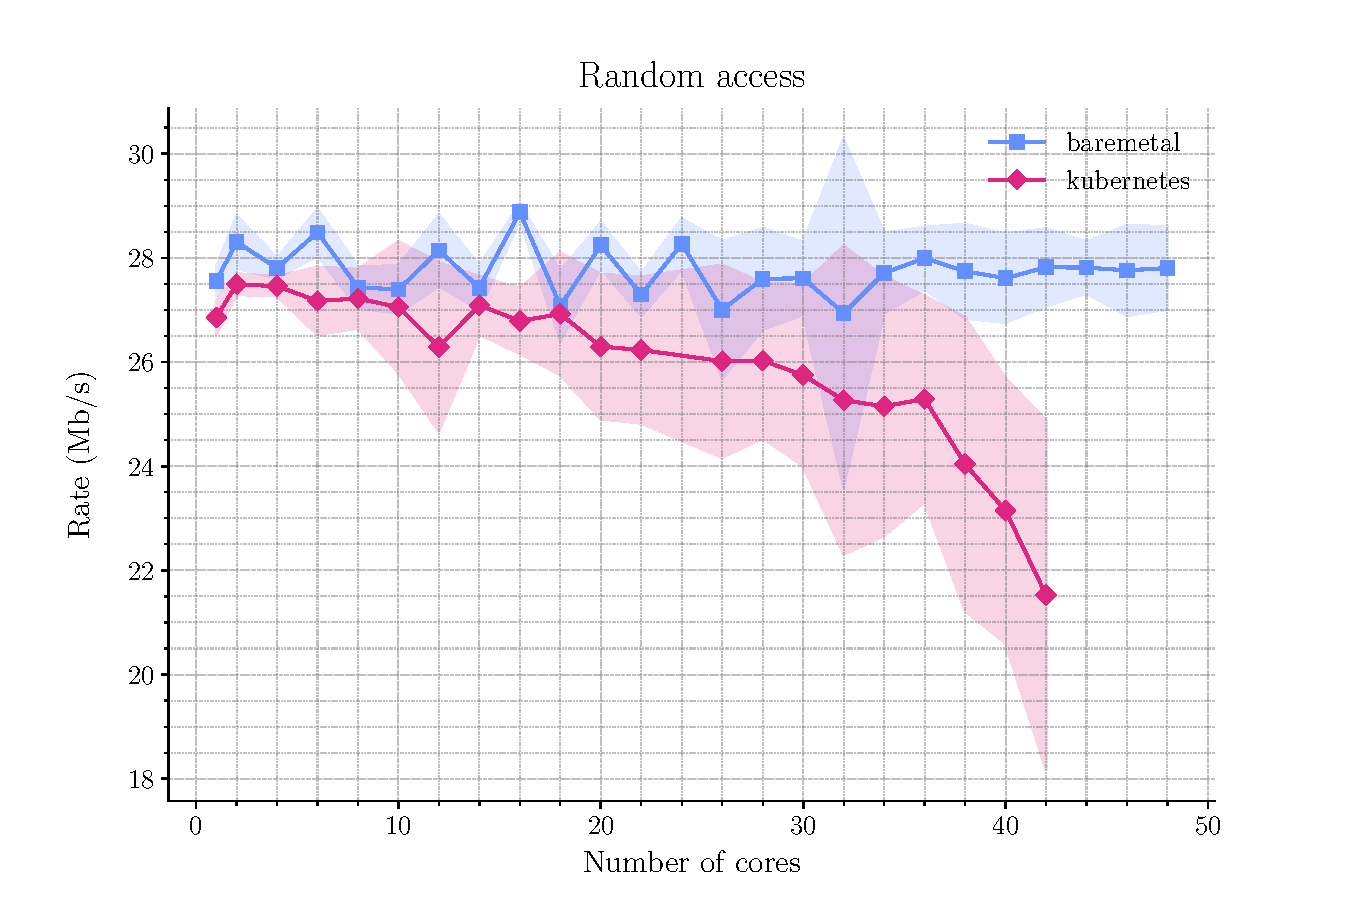
\includegraphics[width=0.9\textwidth]{img/chpt4/array-random-access}
  \caption{Difference in performance between the bare metal case and the
    Kubernetes cluster on the same hardware in retrieving a random element from
    a 2-D array.}
  \label{fig:array-random-access}
\end{figure}

\subsection{Data frames}

The results obtained with the data frames confirm some already known facts.
First, the data frames are the less performant collection of Dask, and the
scaling profile is not as good as the arrays.
Those objects are not meant to be used for numerical computation of large
amounts of data but are more suitable for data manipulation and post-processing
of the results previously obtained in a precedent computation phase.

The outcomes of the different operations executed on the benchmark data frames
are all similar to each other, showing the same trend.
As an example, in figures \ref{fig:dataframe-reduction-std}\footnote{
  Data are available in tables \ref{tab:baremetal-group-by-operation-df} and
  \ref{tab:kube-group-by-operation-df} in appendix \ref{appendix:dask}.
} and \ref{fig:dataframe-sort}\footnote{
  Data are available in tables \ref{tab:baremetal-order-data} and
  \ref{tab:kube-order-data} in appendix \ref{appendix:dask}.
}, that show respectively the performance of the group-by operation and the
sorting of the data frame by a column.

It is possible to appreciate the lack of scalability of the data frames, which
is not determined by a bottleneck caused by the infrastructure but by the very
nature of the data frame object.
Increasing the resources booked for performing those kinds of operations does
not result in a gain in performance.

The other interesting aspect to notice is the systematic tendency of Kubernetes
to be slower compared to the bare metal case.
The overhead introduced by the orchestrator is more relevant in this case, and
the performance gap is more evident than in the array case.
This could be caused by a more significant need amount of communication between
the workers and the scheduler (remember that the data frames are more structured
and heterogeneous, and in Dask every task a worker performs is assigned to it by
the scheduler), which makes weigh more the less efficient communication mangled
by the Kubernetes infrastructure overhead.

\begin{figure}
  \centering
  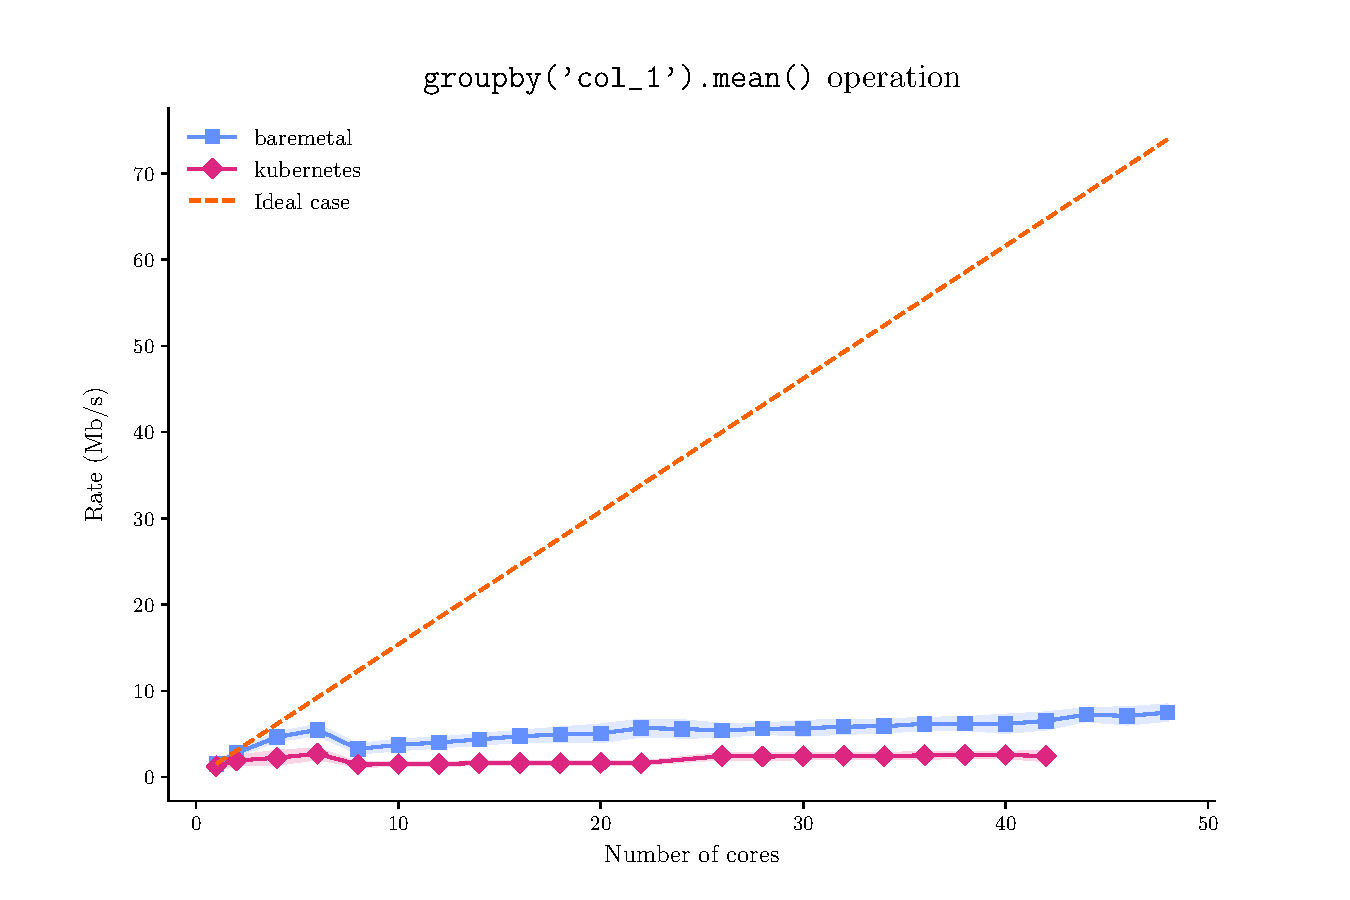
\includegraphics[width=0.9\textwidth]{img/chpt4/df-group-by-operation}
  \caption{Performance variation between the bare-metal environment and the
    Kubernetes cluster on identical hardware when executing a "groupby"
    operation on a single column.}
  \label{fig:dataframe-reduction-std}
\end{figure}

\begin{figure}
  \centering
  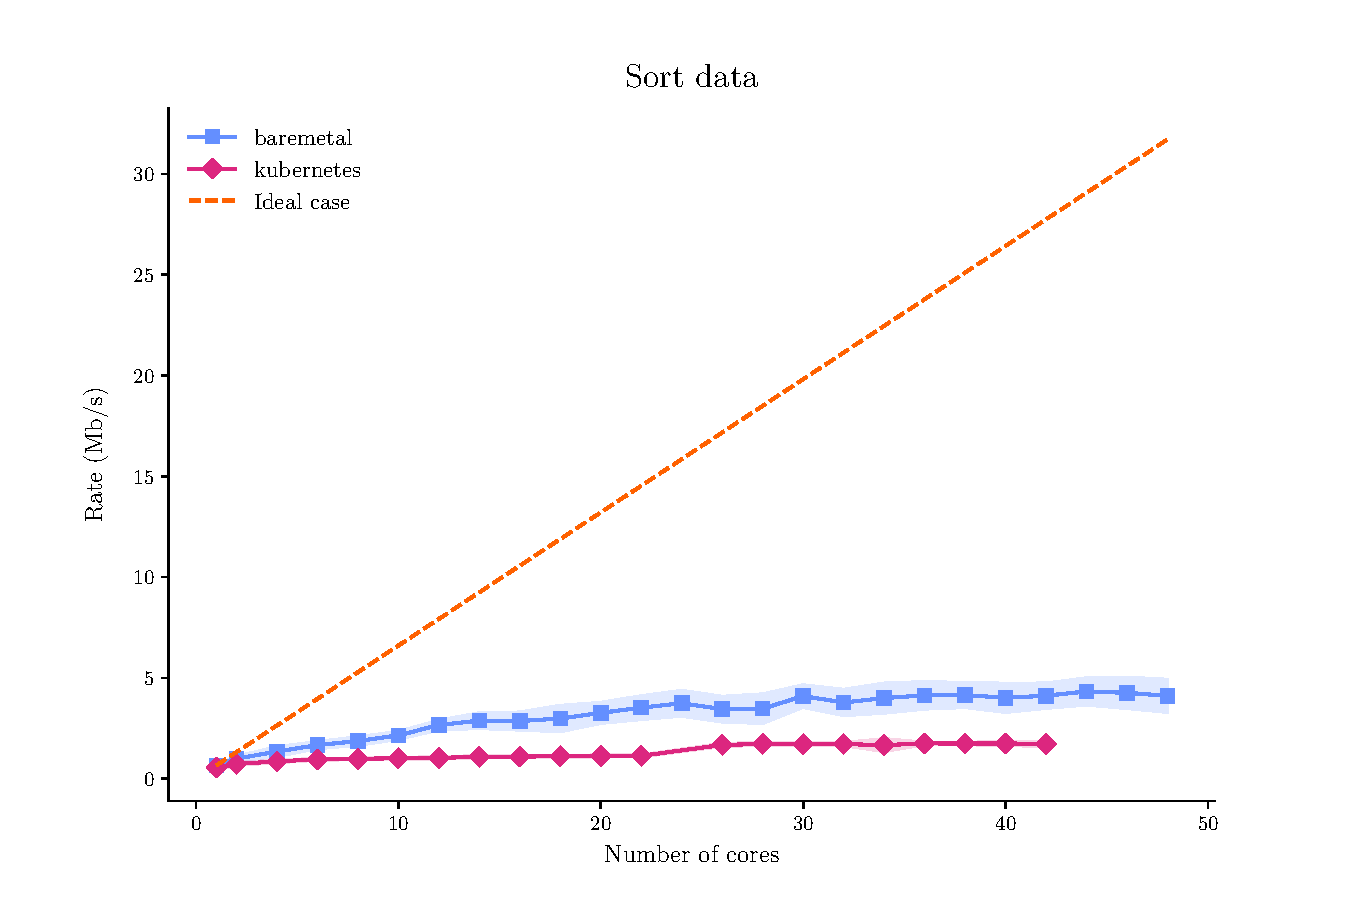
\includegraphics[width=0.9\textwidth]{img/chpt4/df-order-data}
  \caption{Sorting an data frame by a column. Difference between the bare metal
    case and the Kubernetes cluster.}
  \label{fig:dataframe-sort}
\end{figure}

\section{Considerations}

The results obtained from the benchmark are pretty interesting and provide some
insights into the performance of the two different infrastructures.

The first and perhaps most important observation is that the overall performance
of the two setups is quite similar under many conditions.
Specifically, the overhead introduced by the Kubernetes infrastructure appears
to impact the overall performance primarily when communication becomes the
dominant aspect of the operation.
This overhead can be attributed to the network latency in inter-node and
intra-node communications, which is more pronounced in a Kubernetes environment
compared to a tightly coupled HPC cluster.

This is a promising result since it means that for a great variety of cases, in
which the need is to perform some forms of \textit{high throughput computing} or
in general operation not communication bounded, the Kubernetes solution
guarantees the same performance of the traditional HPC setup, with all the
advantages that the containerization and the orchestration bring.

However, on the opposite side, the results obtained in workloads in which
Communication is the dominant aspect and involves frequent data exchange among
different processes.
For example, the sum of the transposed matrix reported has evinced a significant
drop in performance in the Kubernetes setup.
This reduction is due to the overhead introduced by the Kubernetes
infrastructure, and is pronounced enough not to make the container orchestrator
solution a priori the best choice for all the use cases.
In this case, an evaluation of the trade-off between the performance from one
side and the flexibility and the easy-to-use high-level interface from the other
side should be done, and the final decision should vary according to the
importance given to one or the other aspect.

Overall, the findings suggest that while Kubernetes can be a viable alternative
to traditional HPC environments for many computational tasks, its suitability
must be assessed on a case-by-case basis.
Future research could further explore optimization strategies to mitigate these
performance drops, making Kubernetes an even more attractive option for a
broader range of applications.
